\section{LO3: Design Principles vs. Data}

\subsection{Data Preprocessing for Effective Visualization}
Effective visualization begins with thorough data preprocessing. For the Gapminder dataset, which is already fairly clean and structured, hypothetical preprocessing steps could include:

\begin{itemize}
\item \textbf{Handling Missing Values:} Inspecting and addressing missing data points through methods like imputation or exclusion.
\item \textbf{Data Normalization:} Adjusting for factors like inflation, especially for economic indicators like GDP per capita.
\item \textbf{Data Transformation:} Applying transformations, such as logarithmic scaling, to handle skewed distributions in variables like GDP per capita.
\item \textbf{Categorization and Binning:} Grouping continuous variables into categories for analyses requiring aggregated data.
\end{itemize}

These steps ensure the data is ready for visualization, accurately representing the underlying narratives.

\subsection{Visualization Design Choices and Practical Applications}
The design of visualizations for the Gapminder dataset is influenced by the nature of the preprocessed data, with each choice aimed at enhancing the understanding and communication of key data insights:

\begin{itemize}
    \item \textbf{Scatter Plots:} As Li, Martens, and Van Wijk suggest, scatter plots are more effective than parallel plots for visual correlation analysis \cite{liJudgingCorrelationScatterplots2010}. In the Gapminder dataset, scatter plots are used to illustrate correlations such as life expectancy versus GDP per capita. The use of a logarithmic scale, demonstrated in Figure \ref{fig:lo2_scatter_plot}, improves comparability across countries with varying economic statuses.

    \item \textbf{Bar Charts:} For demographic comparisons, such as population distribution across continents, bar charts provide a clear and concise representation. This is exemplified in Figure \ref{fig:lo3_barchart}.

\begin{figure}[h]
    \centering
    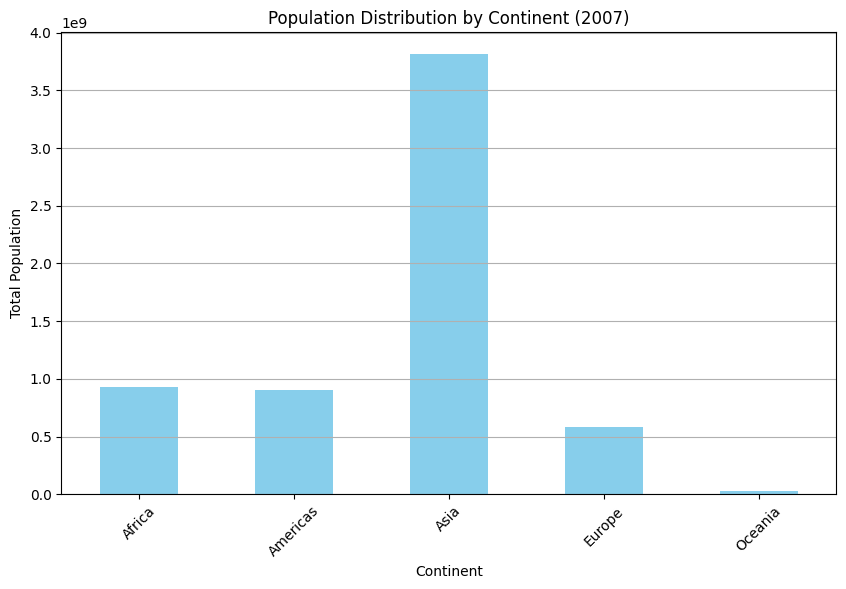
\includegraphics[width=0.8\textwidth]{images/plots/lo3_barplot.png}
    \caption{Bar Chart of Population Distribution Across Continents (2007)}
    \label{fig:lo3_barchart}
\end{figure}

    \item \textbf{Color Schemes:} Appropriate color schemes, as Silva, Santos, and Madeira note, enhance interpretability and appeal \cite{silvaUsingColorVisualization2011}. In the Gapminder visualizations, distinct colors differentiate data categories or geographical regions, aiding in pattern recognition and comparison.

    \item \textbf{Additional Applications:}
\begin{itemize}
    \item \textit{Multidimensional Data Representation:} Bubble charts combine multiple variables into a single plot, offering a nuanced analysis of interrelated factors. For example, Figure \ref{fig:lo2_scatter_plot} shows the relationship between GDP per capita, life expectancy, and population.
    \item \textit{Time Series Analysis:} Line charts track changes over time, revealing trends and patterns in life expectancy or economic growth. This is demonstrated in Figure \ref{fig:lo2_line_chart_w_gaps}.
    \item \textit{Comparing Distributions:} Box plots for different continents allow for a clear comparison of GDP per capita distributions, highlighting economic variations.
    \item \textit{Highlighting Regional Disparities:} Map visualizations underscore geographical disparities, coloring countries based on key indicators like GDP per capita or life expectancy. This is exemplified in Figure \ref{fig:lo2_map}.
\end{itemize}
\end{itemize}

Together, these design choices and applications tailor the visualization techniques to the characteristics of the Gapminder dataset, thereby facilitating a clearer and more impactful data storytelling.

\subsection{Challenges and Adaptations}
In visualizing diverse datasets like Gapminder, challenges such as presenting a wide range of GDP values are common. Adapting visualization techniques, like using logarithmic scales, helps in effectively conveying patterns and outliers. This adaptability underscores the essence of LO3, highlighting the importance of aligning visualization strategies with the nature and requirements of the data.